% $> xelatex emv.redes-neuronales.presentacion.tex
% o bien
% $> lualatex emv.redes-neuronales.presentacion.tex
\documentclass[spanish]{beamer}

\usepackage[es-tabla]{babel}

\usepackage{graphics,tikz}
\usetikzlibrary{automata, positioning, arrows}

\usepackage{pgfplotstable}
\pgfplotsset{compat=1.16}

\usepackage{adjustbox}
\usepackage{booktabs}
\usepackage{multirow}
\usepackage{enumitem}

% Matemáticas

\usepackage{amsmath, amsthm, amssymb}
\usepackage{mathtools}
\usepackage{commath}

%%% FUENTES

\usepackage[no-math]{fontspec}
\setmainfont{Libertinus Serif}
\setsansfont{Libertinus Sans}
\setmonofont{Libertinus Mono}

\usepackage[math-style=TeX]{unicode-math}
\setmathfont{Libertinus Math}

\usepackage{pifont}
\newcommand{\cmark}{\ding{51}}%
\newcommand{\xmark}{\ding{55}}%

%%% COLORES

\definecolor{background}{HTML}{F5F5F4}
\definecolor{foreground}{HTML}{3F3F3F}
\definecolor{strings}{HTML}{ED982C}
\definecolor{operators}{HTML}{CF4818}
\definecolor{identifiers}{HTML}{9A71BA}
\definecolor{keywords}{HTML}{5486C8}
%\definecolor{keywords}{HTML}{54BFC7}
\definecolor{numbers}{HTML}{80951D}
\definecolor{comments}{HTML}{AFAFAF}

%%% LISTINGS

\usepackage{listings}

\lstset{
  numbers=left,
  belowcaptionskip=1\baselineskip,
  basicstyle=\scriptsize\ttfamily\color{foreground},
  keywordstyle=\color{keywords},
  commentstyle=\color{comments},
  stringstyle=\color{strings},
  identifierstyle=\color{identifiers},
  numberstyle=\color{foreground},
  xleftmargin=2em,
  framexleftmargin=1.5em,
  breaklines=true,
  showstringspaces=false,
  tabsize=2
}

% Bibliografía

\usepackage[sorting=none, style=apa, isbn=true]{biblatex}
\DefineBibliographyStrings{spanish}{
  urlseen = {Consultado},
  retrieved = {Consultado},
}
\addbibresource{bibliografia.bib}

%%% AJUSTES DE BEAMER

%\usefonttheme{professionalfonts}

\setlength{\leftmargini}{0cm}
\setlength{\leftmarginii}{2em}

\setbeamertemplate{navigation symbols}{}

\setbeamerfont{title}{series=\bfseries}

%\setbeamertemplate{frametitle}{\color{foreground}\vspace*{1cm}\bfseries\insertframetitle\par\vskip-6pt}
\setbeamerfont{frametitle}{series=\bfseries}
\setbeamercolor{frametitle}{fg=foreground}
\setbeamerfont{framesubtitle}{size=\normalfont\small}
\setbeamercolor{framesubtitle}{fg=foreground}

\setbeamercolor{background canvas}{bg=background}

\setbeamercolor{normal text}{fg=foreground}
\setbeamercolor{alerted text}{fg=foreground}
\setbeamercolor{block title}{fg=foreground}
\setbeamercolor{alerted text}{fg=foreground}

\setbeamercolor{itemize item}{fg=foreground}
\setbeamercolor{enumerate item}{fg=foreground}

\setbeamertemplate{itemize items}[circle]
\setitemize{
  label=\usebeamerfont*{itemize item}
  \usebeamercolor[fg]{itemize item}
  \usebeamertemplate{itemize item}
}

\setbeamercolor*{title}{fg=foreground}
\setbeamercolor{qed symbol}{fg=foreground}

\usebeamercolor[fg]{normal text}

\setbeamertemplate{footline}[frame number]
\setbeamerfont{page number in head/foot}{size=\small}

\setbeamercolor{section in toc}{fg=foreground}
\setbeamerfont{section in toc}{series=\bfseries}

\setbeamercolor{caption name}{fg=foreground}
\setbeamerfont{caption name}{series=\bfseries}

\setbeamercolor{bibliography entry note}{fg=foreground}
\setbeamercolor{bibliography entry author}{fg=foreground!40!black}

\hypersetup{
  colorlinks=true,
  citecolor=numbers,
  urlcolor=operators,
  linkcolor=foreground
}

%%% INFORMACIÓN DEL DOCUMENTO

\title{Redes neuronales artificiales}
\subtitle{Estadística Multivariante}
\author{
  Johanna Capote Robayna\texorpdfstring{\\}{}
  Antonio Coín Castro\texorpdfstring{\\}{}
  Guillermo Galindo Ortuño\texorpdfstring{\\}{}
  José María Martín Luque\texorpdfstring{\\}{}
  Luis Antonio Ortega Andrés\texorpdfstring{\\}{}
  Cristina de la Torre Villaverde
}
\institute{\normalsize Universidad de Granada}
\date{20 de enero de 2020\texorpdfstring{\\}{} \small Curso 2019-2020}

\begin{document}

\maketitle

\begin{frame}{Índice}
  \tableofcontents
\end{frame}

\section{Redes neuronales biológicas}

\begin{frame}{Redes neuronales biológicas}
  \begin{itemize}
    \item Ciencia cognitiva: estudio científico de la mente y sus procesos.
    \item Conexionismo: los fenómenos mentales pueden describirse mediante redes compuestas por unidades sencillas e interconectadas entre sí.
    \item Para entender cómo funciona una red neuronal artificial es útil comprender primero cómo funcionan las redes neuronales biológicas.
  \end{itemize}
\end{frame}

\begin{frame}{Redes neuronales biológicas}
  \begin{itemize}
    \item Neuronas: células básicas que componen el sistema nervioso.
    \item Dos partes diferenciadas: cuerpo celular y axón.
    \item Dendritas: receptores de señales.
    \item Axón: emisor de señales.
  \end{itemize}
\end{frame}

\begin{frame}{Redes neuronales biológicas}
  \begin{figure}[b]
    \centering
    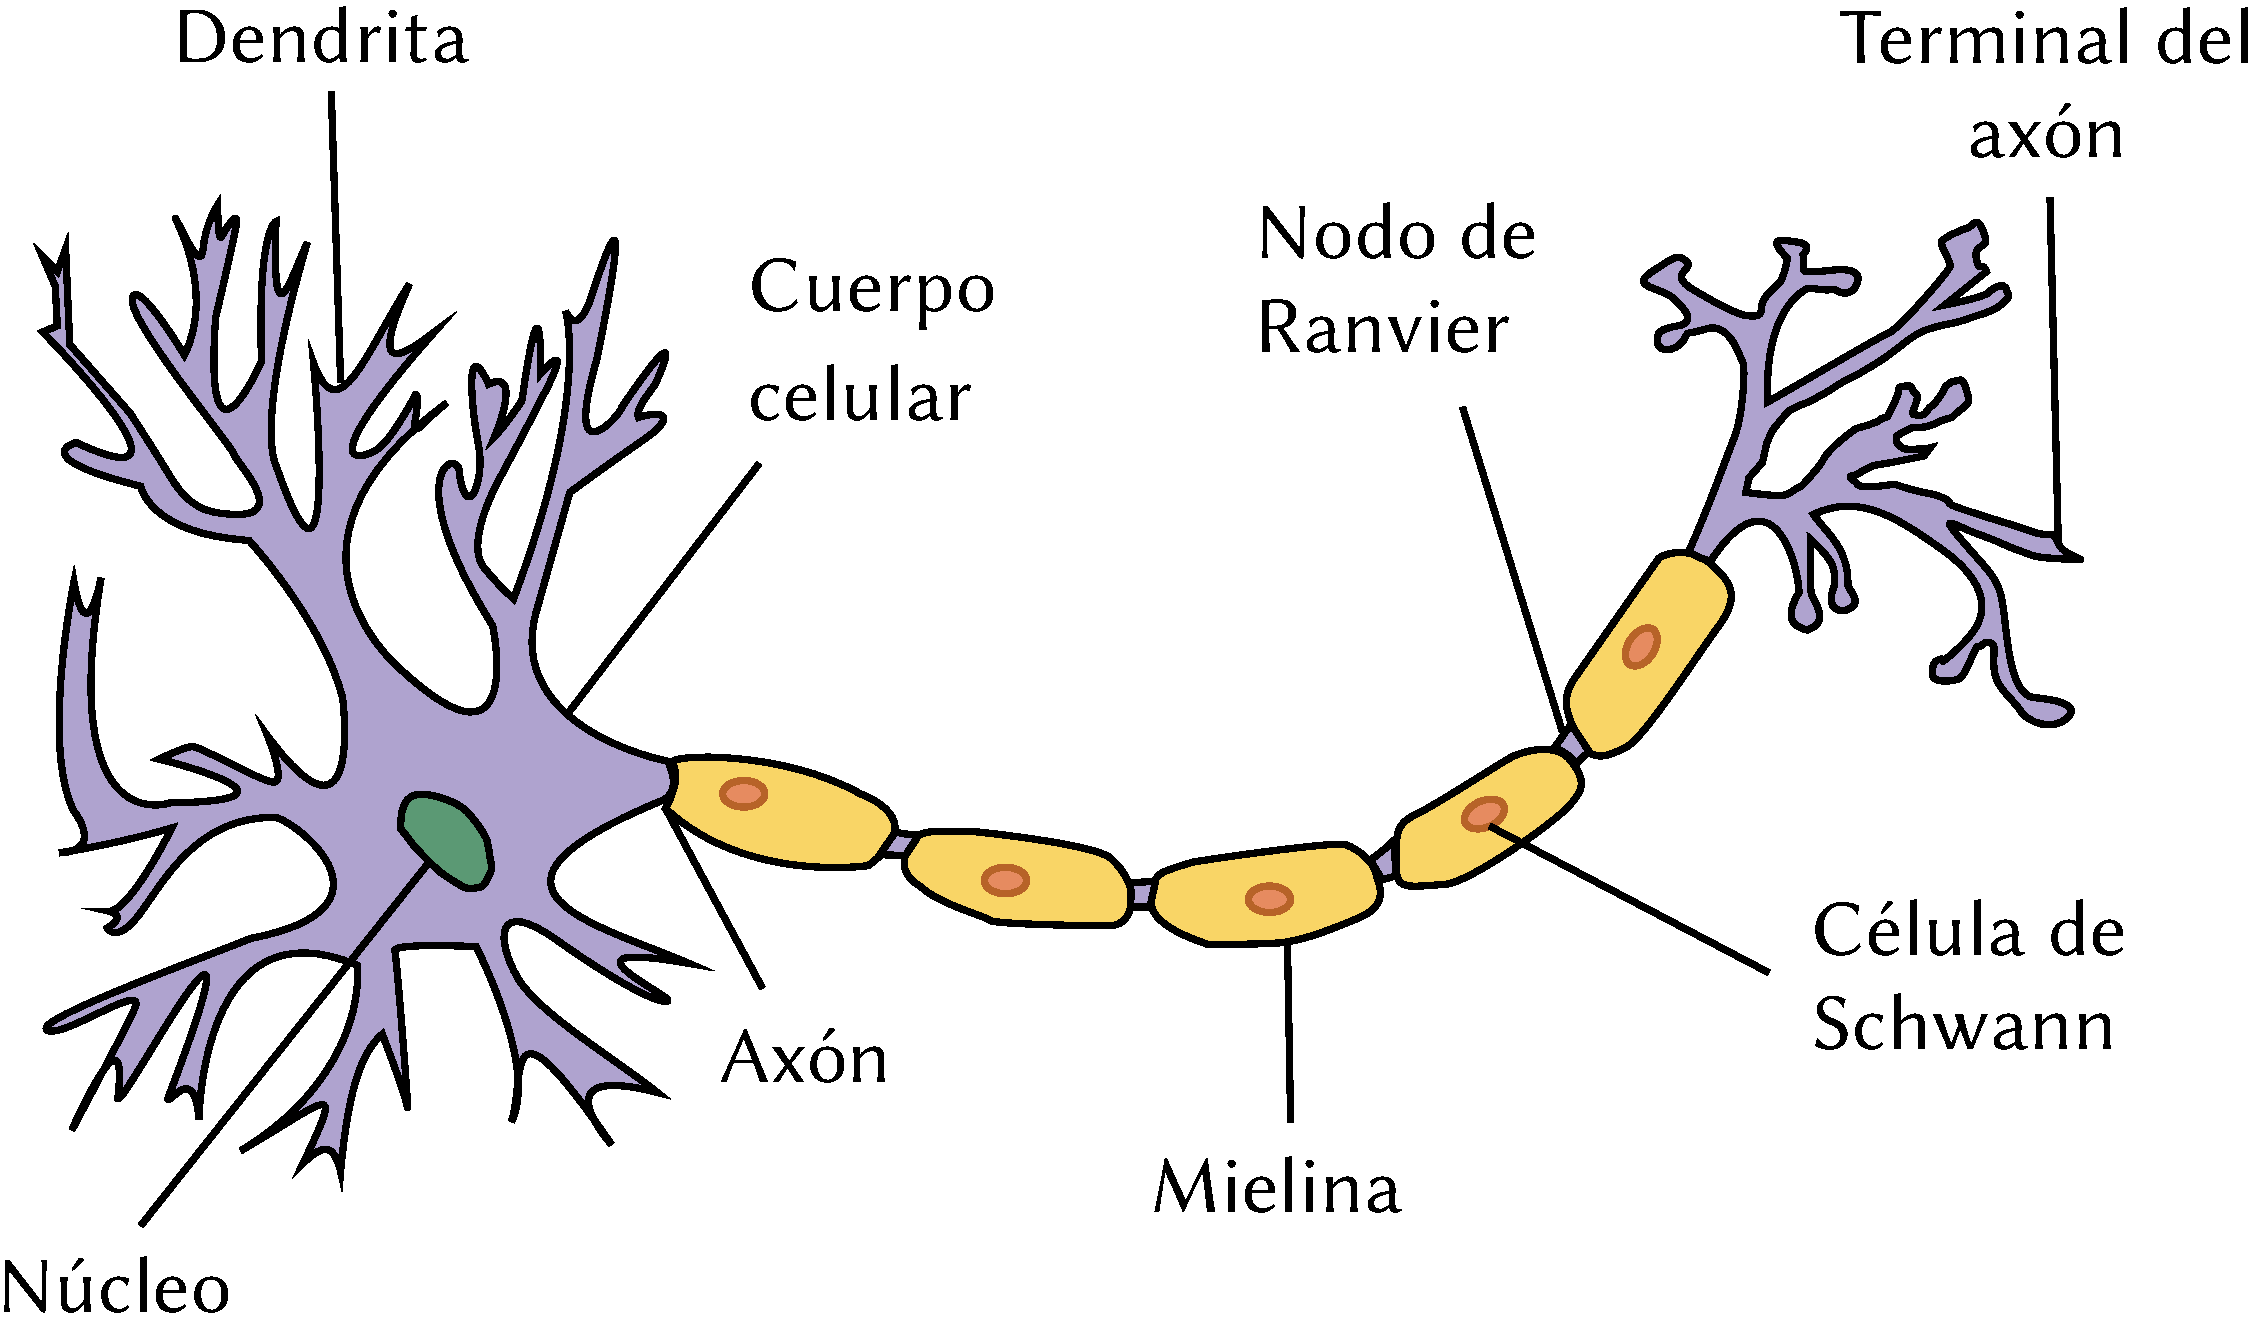
\includegraphics[width=0.7\textwidth]{img/neurona}
    \caption{Estructura de una neurona. Basada en \parencite{dhp1080_neurona_2007}.}
    \label{fig:neurona}
  \end{figure}
\end{frame}

\begin{frame}{Redes neuronales biológicas}
  \begin{itemize}
    \item Las neuronas se envían señales entre sí mediante un proceso electroquímico denominado sinapsis.
    \item La neurona presináptica (emisora) libera los neurotransmisores a través del axón y la neurona postsináptica (receptora) los capta a través de las dendritas.
    \item La tasa de envío por parte de la neurona presináptica depende de la proporción de dos tipos de sinapsis que esta reciba: \begin{itemize}
      \item sinapsis inhibidoras,
      \item sinapsis excitadoras.
    \end{itemize}
  \end{itemize}
\end{frame}

\section{Estructura y funcionamiento de las redes neuronales}

\begin{frame}{Neurona de McCulloch-Pitts}
  \begin{itemize}
    \item Modelo computacional. Múltiples entradas a una unidad de procesamiento y una sola salida.
    \item Cada entrada puede tomar el valor 0 o 1 y puede ser de tipo excitador o inhibidor. \begin{itemize}
      \item Si alguna de ellas es inhibidora y transmite el valor 1, la salida es 0.
      \item Si no hay conexiones inhibidoras activadas, se suman las entradas. Si dicha suma es mayor que el valor umbral, la salida es 1, en otro caso, 0.
    \end{itemize}
  \end{itemize}
\end{frame}

\begin{frame}{Neurona de McCulloch-Pitts}
  \begin{figure}[h]
    \centering
    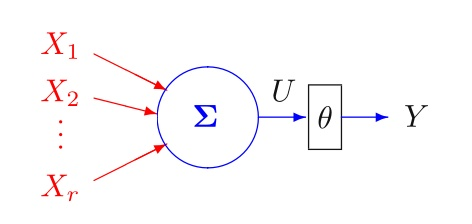
\includegraphics[width=.7\textwidth]{img/mcculloch-pitts}
    \caption{Neurona de McCulloch-Pitts con $r$ entradas binarias $X_1,\dots,X_r$, una salida binaria $Y$ y un umbral $\theta$. Extraída de \parencite{izenman_modern_2008}.}
    \label{fig:mcculloch-pitts}
  \end{figure}
\end{frame}

\begin{frame}{Neurona de McCulloch-Pitts}
  \begin{itemize}
    \item Este modelo no es adecuado para realizar un proceso de aprendizaje ya que hay que cambiar los valores de la neurona para resolver diferentes problemas.
    \item Se perdió pronto el interés en este modelo computacional y se desarrollaron otros.
  \end{itemize}
\end{frame}

\begin{frame}{Perceptrón de una capa}
  \begin{itemize}
    \item El perceptrón es un sistema que imita el funcionamiento de una neurona, consistente en una neurona de \textit{McCulloch-Pitts} con pesos $\beta_i \in \mathbb{R}$
    \item $\beta_i > 0$ conexiones exitadoras.
    \item $\beta_i < 0$ conexiones inhibidoras.
    \item $U \sum_j \beta_j X_j$
  \end{itemize}
  \begin{figure}[h]
    \centering
    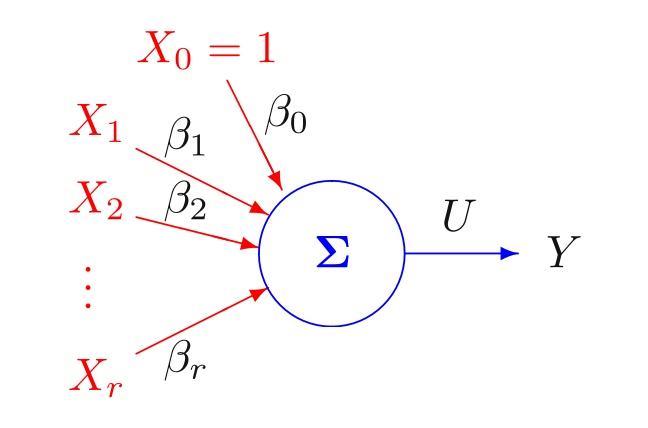
\includegraphics[width=.7\textwidth]{img/perceptron}
  \end{figure}
\end{frame}

\begin{frame}{Perceptrón de una capa}
  \begin{itemize}
    \item Linealmente separables: se puede interpretar como un algoritmo de clasificación binaria.
    \item No linealmente separables: la función asociada no es computable por un Perceptrón.
  \end{itemize}
  \begin{figure}[h]
    \centering
    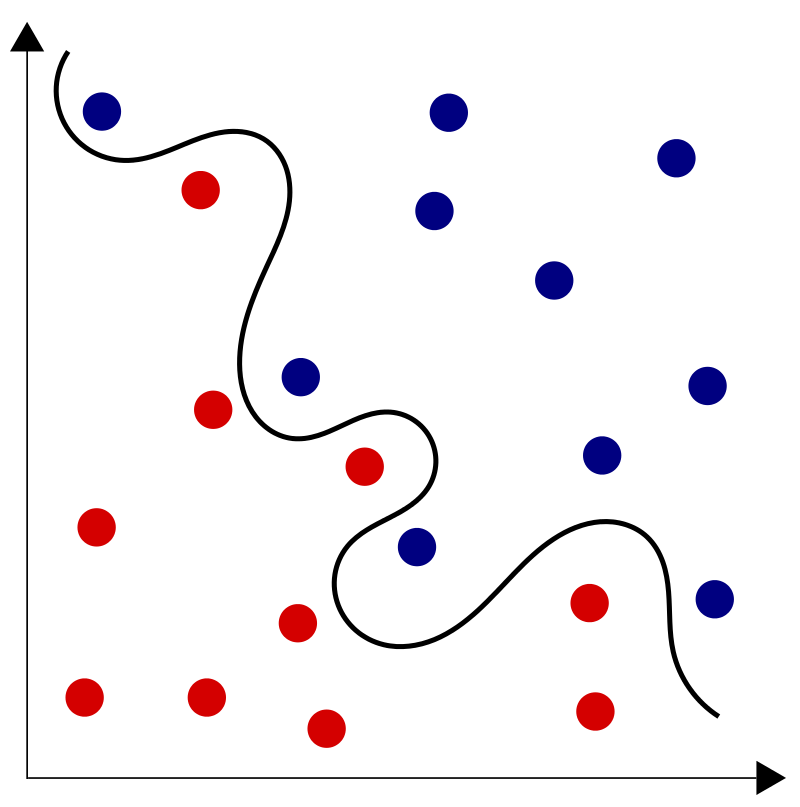
\includegraphics[width=.2\textwidth]{img/non-separable}
    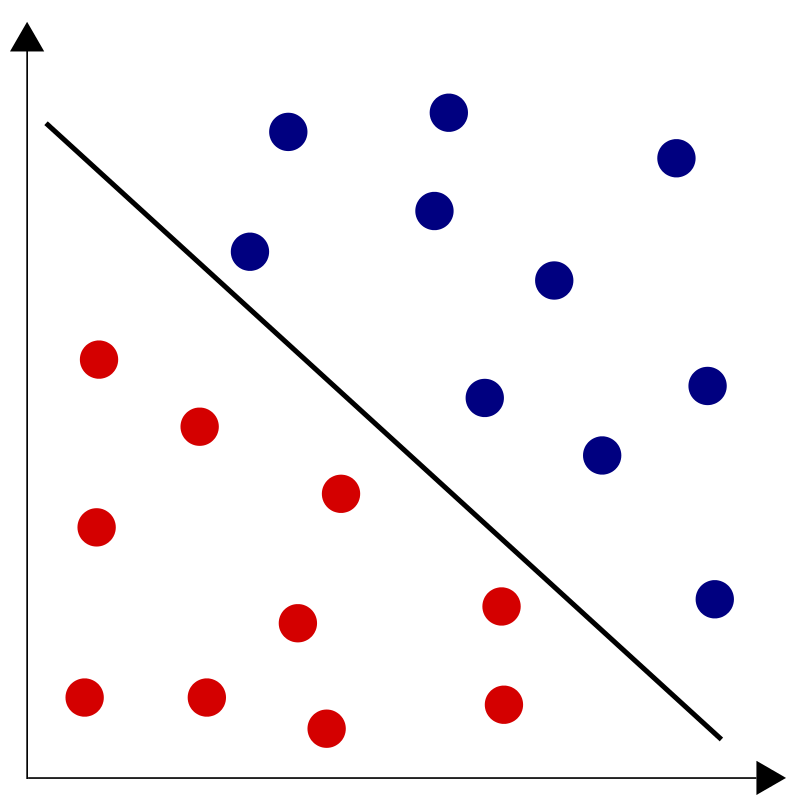
\includegraphics[width=.2\textwidth]{img/separable}
  \end{figure}
\end{frame}

\begin{frame}{Funciones de activación}
  \begin{itemize}
    \item Entrada: $X=(X_1, \cdots , X_r)^T$ vector aleatorio de entradas y tenemos $s$ nodos de salida, en cada uno de ellos se calcula:
    $$U_k = \beta_{0k} + X^T \beta_{k} , \ k = 1, \cdots , s $$
    \item Salida: $$ U_k = f(\beta_{0k} + X^T \beta_k) \ k = 1, \cdots , s$$
  \end{itemize}
  \begin{figure}[h]
    \centering
    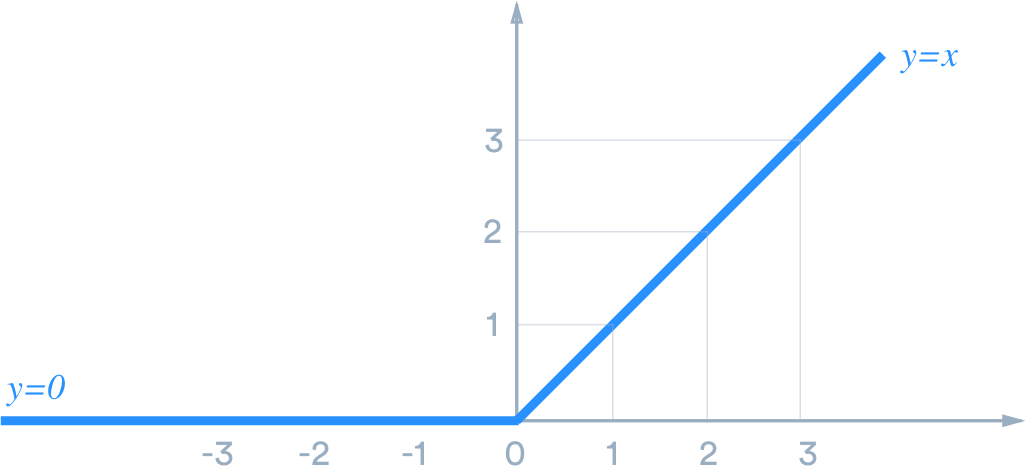
\includegraphics[width=.7\textwidth]{img/relu}
    \caption{Gráfica de la función ReLU.}
  \end{figure}
\end{frame}

\begin{frame}{Procesos de aprendizaje}
\begin{itemize}
\item La estrategia de las redes es utilizar el conocimiento de la clase correcta para ir pasando ejemplos por la red y predecir la clase a la que pertenece cada uno, intentando corregir los pesos si se detecta un error. Esta técnica se conoce como \textbf{aprendizaje supervisado}.
\item La regla para actualizar los pesos en cada iteración es la siguiente:
  \begin{enumerate}
    \item Si la versión actual de los pesos $\beta_h$ consigue clasificar correctamente $X_h$, no cambiamos los pesos para la siguiente iteración.
    \item Si con los pesos $\beta_h$ no obtenemos una clasificación correcta, hacemos:
    $$\beta_{h+1} = \beta_h + \eta signo(X^{t}_{h} \beta_h)X_h  $$
  \end{enumerate}
  El parámetros $\eta > 0$ se conoce como \textit{learning rate}.
\end{itemize}
\end{frame}

\begin{frame}{Procesos de aprendizaje}
\item Una solución del problema será un vector de pesos $\beta^\ast$ que clasifique correctamente todos los ejemplos. Y de aquí obtenemos el siguiente resultado:
\item \textbf{Teorema (Convergencia del perceptrón)} Para un problema de clasificación binaria con clases linealmente separables, si existe una solución $\beta^\ast$, el algoritmo descrito anteriormente la encontrará en un número finito de iteraciones.
\end{frame}

\begin{frame}{Perceptrón multicapa}
  \begin{itemize}
    \item Se distribuyen los nodos en varias capas y se aplican transformaciones no lineales en el paso de una capa a la siguiente.
    \item Dos tipos:
    \begin{itemize}
      \item Capas totalmente contectadas.
      \item Capar parcialmente conectadas.
    \end{itemize}
  \end{itemize}
  \begin{figure}[h]
    \centering
    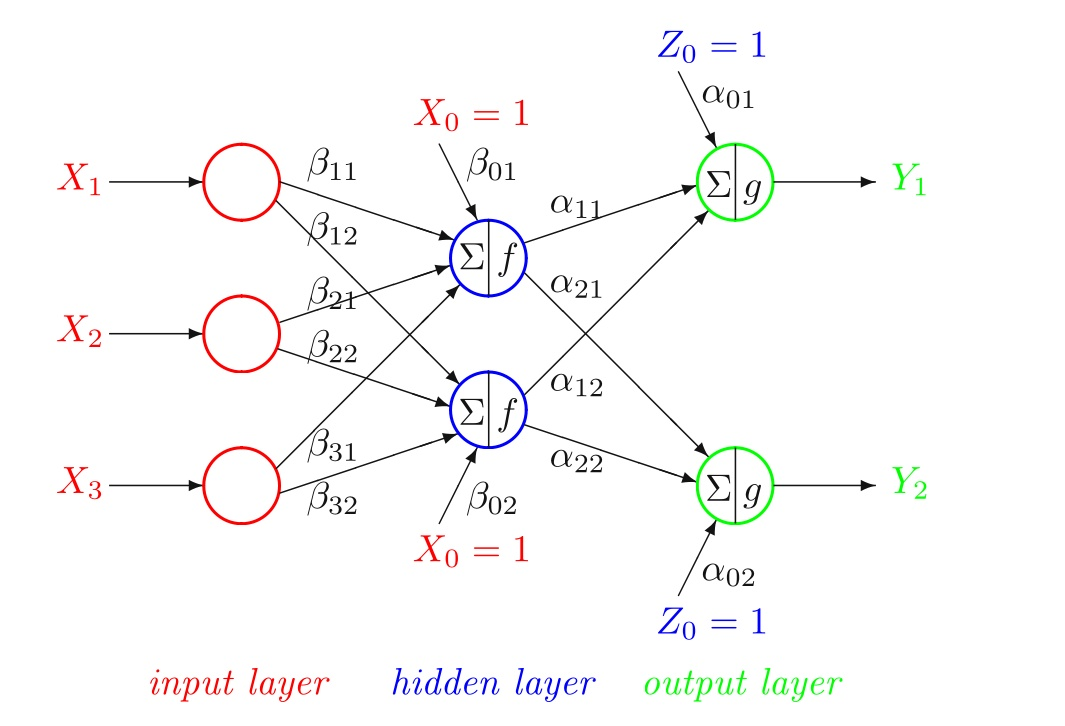
\includegraphics[width=.7\textwidth]{img/multicapa}
  \end{figure}
\end{frame}

\begin{frame}{Perceptrón multicapa}
  \begin{itemize}
    \item Para el proceso de aprendizaje de la red, se utiliza la técnica de gradiente descendente.
    \item Una vez conseguida pesos \textit{suficientemente buenos} se puede utilizar la red para clasificar nuevos ejemplos.
    \item También se puede abordar el problema de regresión lineal.
    \item Desventaja: pérdida de interpretabilidad frente a modelos clásicos.
    \item Ventaja: consiguen resolver problemas mucho más complejos.
  \end{itemize}
\end{frame}

\begin{frame}{Principales problemas}
\textbf{Overfitting}: La red ha memorizado los ejemplos de capacitación, pero no ha aprendido a generalizar a nuevas situaciones.
  \begin{figure}[h]
    \centering
    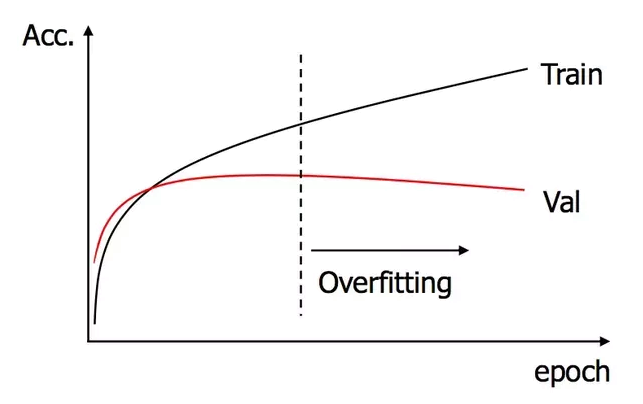
\includegraphics[width=.6\textwidth]{img/overfitting}
  \end{figure}
\end{frame}
\begin{frame}{Principales problemas}
\textbf{Learning rate}: Indica cuanto hay que cambiar el modelo en respuesta al error estimado cada vez que actualizan los pesos de este.
  \begin{figure}[h]
    \centering
    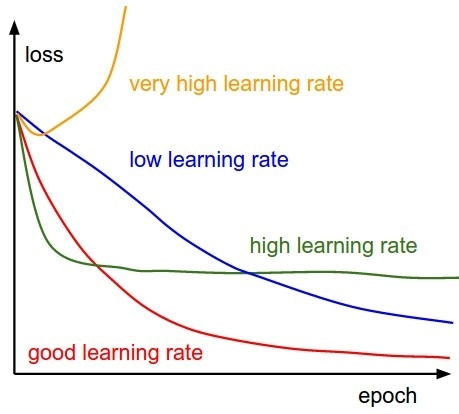
\includegraphics[width=.6\textwidth]{img/learning-rate}
  \end{figure}
\end{frame}

\begin{frame}{Teorema de aproximación universal}
El teorema de aproximación universal establece que una red feed-forward con una sola capa oculta que contiene un número finito de neuronas puede aproximarse a funciones continuas en subconjuntos compactos de $R_n$, bajo condiciones poco restrictivas sobre la función de activación.
Dos tipos:
\begin{itemize}
  \item Ancho acotado.
  \item Ancho no acotado.
\end{itemize}
\end{frame}

\begin{frame}{Clasificación de redes neuronales}
\begin{itemize}
  \item \textbf{Aprendizaje supervisado}. El trabajo de la red consiste en reproducir la salida deseada para cada entrada, minimizando el cuadrado de la distancia entre la salida de la red y la salida esperada.
  \item \textbf{Aprendizaje no supervisado}. Los datos de entrada se dan junto con una función de coste (una función de los datos y la salida de la red). El objetivo de la red es minimizar dicha función de coste.
  \item \textbf{Aprendizaje por refuerzo}. El objetivo de este tipo de entrenamiento es hacer que la red adapte una política de acción que minimice un coste (\textit{long-term}).
\end{itemize}
\end{frame}

\begin{frame}{Redes convolucionales}
  \begin{itemize}
    \item Convolución: consiste en «desplazarse» por todas las posibles posiciones de una matriz, y aplicar el producto elemento a elemento entre la submatriz y el filtro seleccionado.

    \begin{figure}[h]
      \centering
      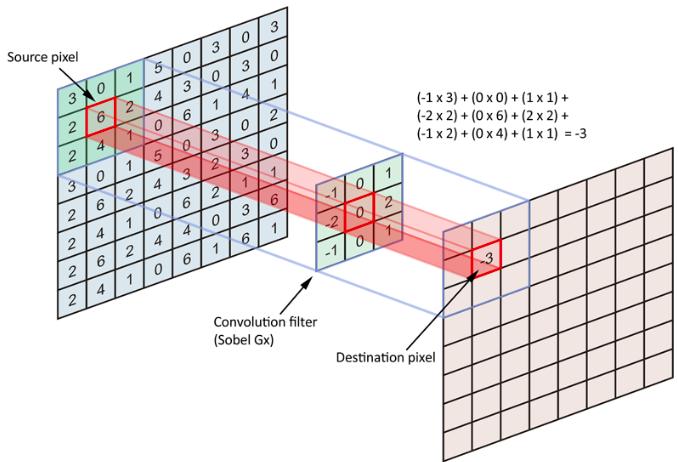
\includegraphics[width=.6\textwidth]{img/conv}
    \end{figure}
  \end{itemize}
\end{frame}

\begin{frame}{Autoencoders}
\begin{itemize}
  \item Un autoencoder es un tipo de read neuronal de aprendizaje no supervisado que aprende a copiar su entrada en la salida. Está formado por dos partes:
  \begin{itemize}
    \item Codificador. Conjunto de capas que transforman la entrada al «código».
    \item Decodificador. Conjunto de capas que transforman el «código» a la entrada original.
  \end{itemize}
\end{itemize}
\begin{figure}[h]
  \centering
  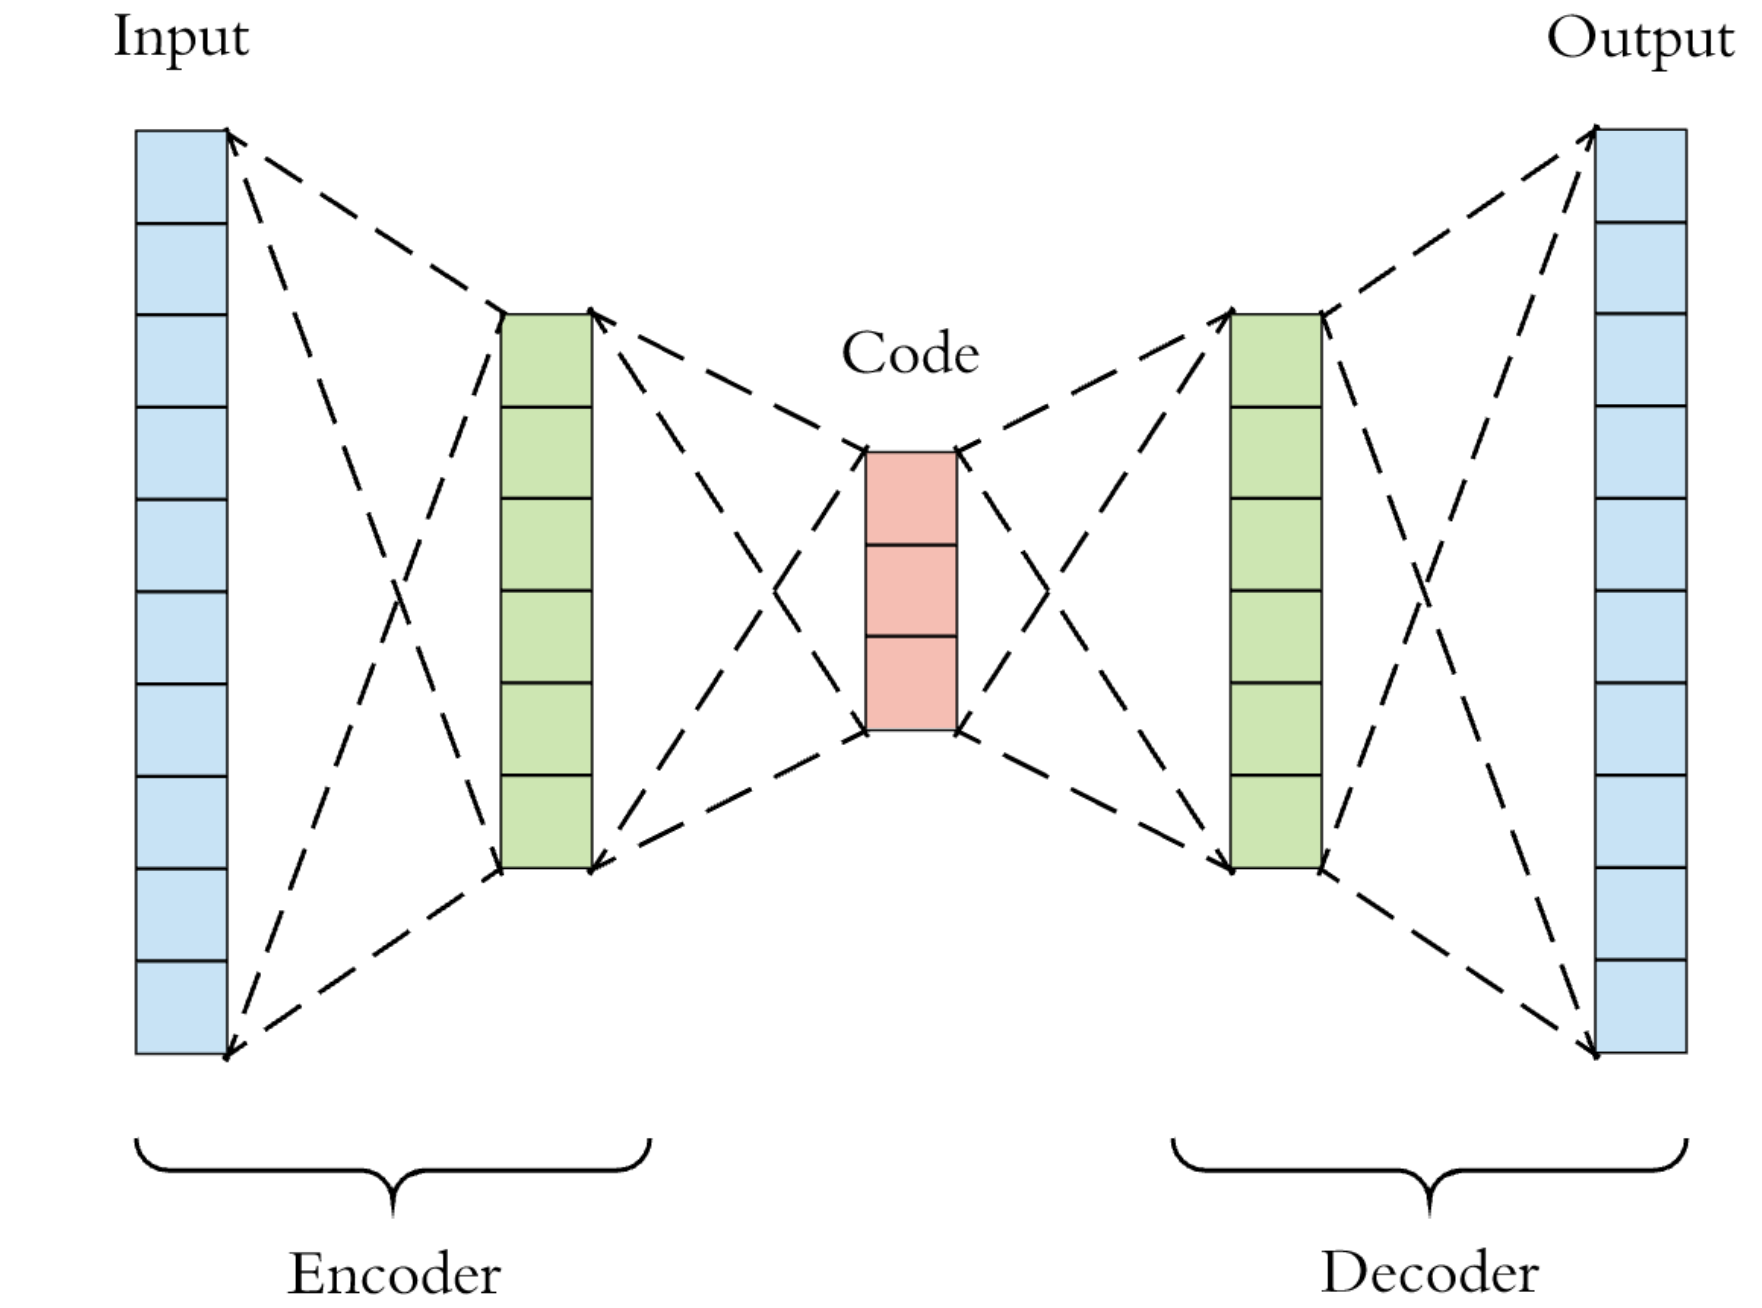
\includegraphics[width=.6\textwidth]{img/autoencoder}
\end{figure}
\end{frame}

\begin{frame}{Redes Neuronales Recurrentes}
\begin{itemize}
\item Son una de las variantes de redes más importantes utilizadas en procesamiento
de lenguaje natural.
\begin{figure}[h]
  \centering
  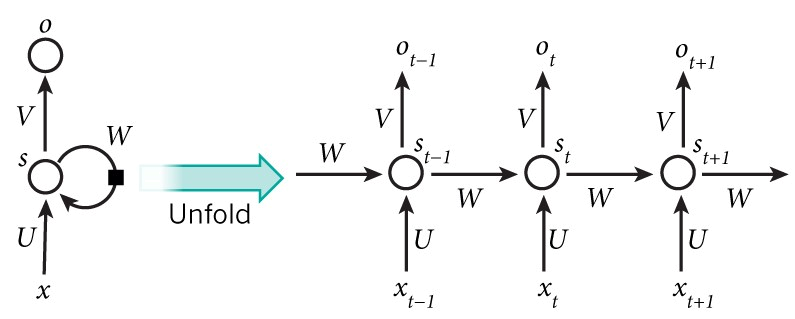
\includegraphics[width=.6\textwidth]{img/rnn}
\end{figure}
\end{itemize}
\end{frame}

\begin{frame}{Ejemplo}
\begin{figure}[h]
  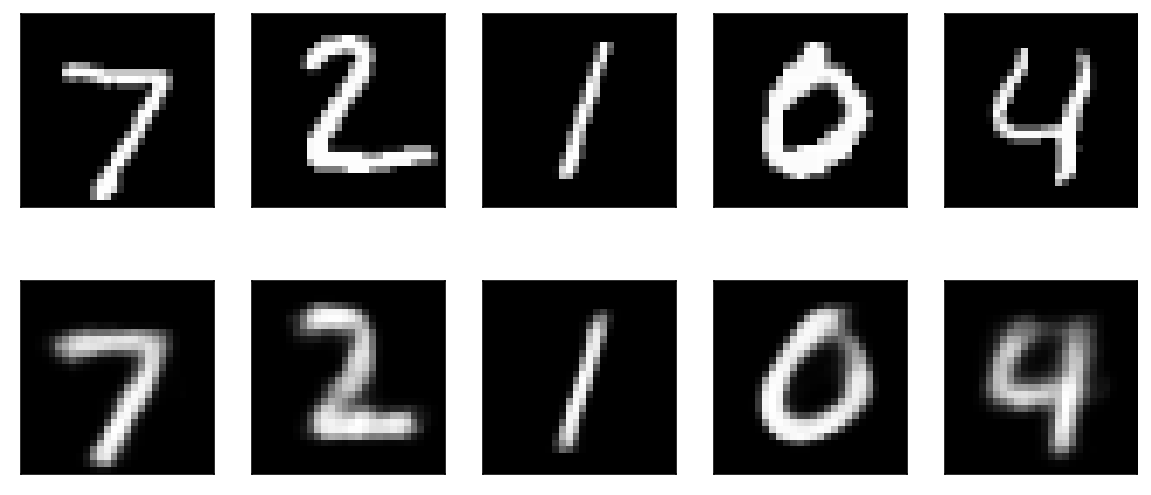
\includegraphics[width=.6\textwidth]{img/autoencoder_ex1}
  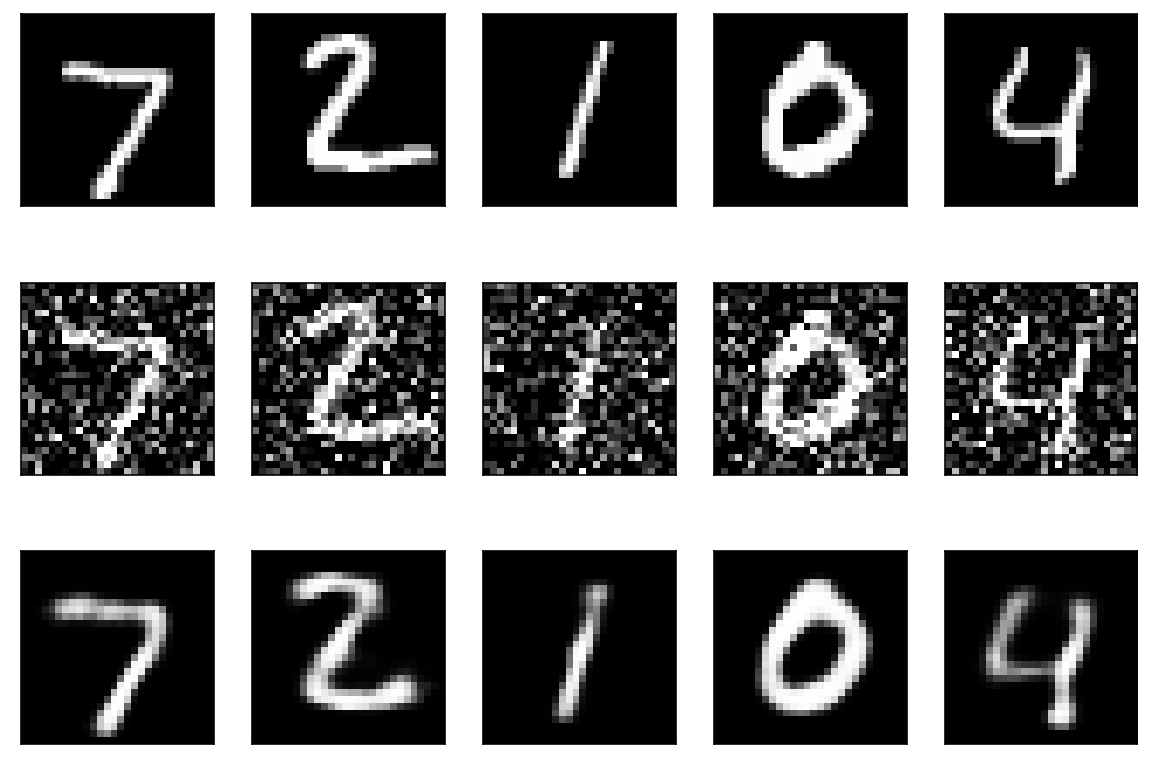
\includegraphics[width=.6\textwidth]{img/autoencoder_ex2}
\end{figure}
\end{frame}

\begin{frame}{CIFAR-10}
\begin{itemize}
  \item El conjunto de datos CIFAR-10 tiene 60000 imágenes en color de 32x32 píxeles divididas en 10 clases, con 6000 imágenes por clase. El conjunto se divide en 50000 imágenes para el conjunto de entrenamiento y 10000 imágenes en el conjunto de test.
  \begin{figure}[h]
    \centering
    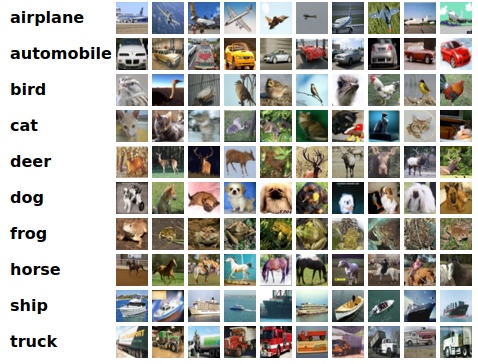
\includegraphics[width=.6\textwidth]{img/cifar10}
  \end{figure}
\end{itemize}

\end{frame}

\begin{frame}[t,allowframebreaks]{Referencias}
  \printbibliography[heading=none]
\end{frame}

\end{document}
